\documentclass[bibliography=totocnumbered]{scrartcl}
\usepackage{imakeidx}
\usepackage{ragged2e}
\usepackage{setspace} % Um den Zeilenabstand zu ändern.
\usepackage{gensymb}
%\usepackage{authblk}
% \usepackage{minitoc} % for the chpaters
\usepackage{wasysym}
%\usepackage{SI}
\usepackage{array} % Verwendung von Matrizen
\usepackage{booktabs} % Schöne Tabellen beziehungsweise sie sehen damit professioneller aus.
\usepackage{tabulary} % Ähnlich wie tabularx, ermöglicht aber das ändern der Ausrichtung der Spalten.
\usepackage{tabularx} % Tabellen mit automatischen Zeilenumbruch.
\usepackage{enumitem}
\usepackage{physics}
\usepackage[T1]{fontenc}% fontec und inputenc ermöglichen
\usepackage{graphicx}%Für Grafiken
\usepackage{rotating} % lässt Grafiken rotieren
\usepackage{mathtools}% mathematische Werkzeuge
\usepackage{amsmath}% Mathetools
\usepackage{amsfonts}% Mathetools
\usepackage{amssymb}% Symbole wie Natürliche Zahlen
\usepackage{geometry}
%\usepackage{bibtex} 
\usepackage{tablefootnote}% Fußnoten in Tabellen
\usepackage{float}% für eingebundene Bilder
\usepackage{fancyhdr} % Seiten schöner gestalten, insbesondere Kopf- und Fußzeile
\usepackage{ulem} 
\usepackage{dcolumn}% Align table columns on decimal point
\usepackage{bm}% bold math
\usepackage[ngerman]{babel} % Worttrennung nach der neuen Rechtschreibung und deutsche Bezeichnungen. babelfunktion wird wegen Literatur gebraucht.
\usepackage{subfloat} % Was macht diese Packet?
\usepackage{caption} % Unter-/Überschriften für Bilder, Grafiken und Tabellen
\usepackage{subcaption}
\usepackage{txfonts}
\usepackage{titling}% Titel
\usepackage[style=alphabetic]{biblatex} %biblatex mit alphabetic laden. alphbetic=Zitationsstil
\usepackage{bookmark}
\usepackage[printonlyused]{acronym}
\usepackage{amsthm}
\usepackage{pdfpages}
\usepackage{tikz}
\usepackage[siunitx,americanvoltages, europeanresistors,americancurrents]{circuitikz}
\usepackage{listings}
\usepackage{abstract}
\usepackage[per-mode = fraction]{siunitx}
\usepackage{hyperref}
\newcommand{\R}{\mathbb{R}} % reelle Zahlen
\newcommand{\N}{\mathbb{N}} % natürliche Zahlen
\newcommand{\C}{\mathbb{C}} % komplexe Zahlen
\newcommand{\Q}{\mathbb{Q}} % rationale Zahlen
\newcommand{\Z}{\mathbb{Z}} % ganze Zahlen
\newcommand{\F}{\mathbf{F}} % Kraft
\newcommand{\E}{\mathbf{E}} % Energie
\newcommand{\V}{\mathbf{v}} % Geschwindigkeit
\newcommand{\B}{\mathbf{B}} % magnetischer Fluss
\newcommand{\J}{\mathbf{j}} % Stromdichte ?
\newcommand{\D}{\mathbf{D}} % elektrische Induktion
\newcommand{\HH}{\mathbf{H}} % magnetische Feldstärke
\newcommand{\M}{\mathbf{M}} % Magnetisierung
\newcommand{\p}{\mathbf{P}}
\newcommand{\rr}{\mathbf{r}}
\newcommand{\vp}{\varphi}
\newcommand{\ve}{\varepsilon}
\newcommand{\vcc}[1]{\left(\begin{matrix}#1\end{matrix}  \right)}
\newcommand{\m}[1]{\left\lbrace #1\right\rbrace}
\newcommand{\los}{\noindent\textbf{Lösung}:}
\newcommand{\rang}[2]{\text{Rang}(#1)=#2}
\newcommand{\vpe}{\frac{1}{4\pi\ve_0}}
\newcommand{\qvpe}{\frac{q}{4\pi\ve_0}}
\newcommand{\geg}{\ac{geg.}}
\newcommand{\ges}{\ac{ges.}}

\newcommand{\kommando}[1]{$\backslash$\textit{#1}}
\newcommand{\com}[1]{$\backslash$\textit{#1}$\left\lbrace\ldots\right\rbrace$}
\newcommand{\Com}[2]{$\backslash$\textit{#1}$\left\lbrace #2\right\rbrace$}
\newcommand{\NeuKommando}[2]{$\backslash \textit{#1} \left\lbrace \backslash \textit{#2}\right\rbrace$}
\newcommand{\latex}{\LaTeX $\;$}


% si unitx
\DeclareSIUnit\litre{l}

\hypersetup{
	colorlinks=true,
	linkcolor=blue,
	filecolor=magenta,      
	urlcolor=cyan,
	citecolor=lime!50!black,
	filecolor=red
}
%\addbibresource{} %Bibliographiedateien laden
\addbibresource{bib.bib}

\geometry{a4paper, left=25mm, right=25mm, top=30mm, bottom=30mm}
\lhead{\thedate}
\rhead{GPR}
\lhead{\thetitle}
\pagestyle{fancy}

\usetikzlibrary{patterns}
\usetikzlibrary{3d}
\makeindex[title=Stichwortverzeichnis,intoc
,options= -s Index-Formatierung.ist
]
\author{Ben J. F.}
\allowdisplaybreaks

\lstset
{ %Formatting for code in appendix
    basicstyle=\footnotesize,
    numbers=left,
    stepnumber=1,
    showstringspaces=false,
    tabsize=2,
    breaklines=true,
    breakatwhitespace=false,
}

\date{03.08.2021}

\title{M5 \\ Oberflächenspannung}

\pagestyle{fancy}
\rfoot{M5}

\begin{document}
	\newgeometry{left=14mm, right=13.5mm, top=60mm, bottom=30mm}
	\begin{titlepage}
		\begin{center}
			{\huge{Grundpraktikum}}\\\vspace*{15mm}
			{\huge{\textbf{\thetitle}}}\\\vspace*{20mm}
			{\theauthor}\\\vspace*{10mm}
			{\thedate}\\\vspace*{20mm}
			
			\vspace{1.5cm}
			\begin{abstract}
			Ziel des Versuches ist es, die Oberflächenspannung $ \sigma $ mittels Bügelmethode zu bestimmen. Zudem werde ich die Feder-Waage kalibrieren. Der Versuch wurde vollständig durchgeführt werden, jedoch konnte ich aufgrund der Zeitknappheit die Kappilarsteighöhenmethode nicht durchführen.
			\begin{table}[H]
			\centering
				\begin{tabular}{|l||c|}
				\hline
				& Platz 4 \\
				\hline
				\hline
				Bügelmethode [mN$ \cdot $m$ ^{-1} $ ]& $\sigma=(65 \pm 6)$ \\
				\hline
				Federkonstante Hinweg & $k=1.28 \pm 0.04$ \\
				\hline
				Federkonstante Rückweg & $k= 1.235 \pm 0.023 $ \\
				\hline
			\end{tabular}
		\end{table}
			
			\end{abstract}
			
			
		\end{center}
	\end{titlepage}
	\makeatother
	\restoregeometry
	\newpage
	
	\tableofcontents
	
	
	\listoffigures 
	\listoftables
	\newpage
	
	
	\section{Versuchsbeschreibung}
	% Versuchziel: Was will ich mit dem Versuch erreichen?
	% Aufgabenstellung
	% theoretische Einführung: Wie sieht die Physik dahinter aus (Knapp fassen)? Welche Formeln verwende ich? Wie ist der Versuch aufgebaut (Skizze, Abbildungen etc)? Welche Einheiten kommen vor?
	Der Versuch hat zweierlei Ziele: Zum einen die Kalibration der Feder-Waage und die Messung der Oberflächenspannung $ \sigma $: 
	\begin{equation}\label{eq: Oberflächenspannung}
		\sigma=\dfrac{\Delta W}{\Delta A}=\dfrac{F}{l}
	\end{equation}
	
	Für die Messung der Oberflächenspannung gibt es zwei Methoden: einmal die Bügelmethode und einmal die Kapillarsteighöhenmethode. Weitere Möglichkeiten die Oberflächenspannung zu messen, werden in Kap. (\ref{sect: Frage 3}) aufgeführt. Aufgrund der knappen Zeit wurde nur die Bügelmethode durchgeführt.


	
	
	\subsection{Bügelmethode} \label{sect: Bügelmethode}
	Der Versuchsaufbau für die Bügelmethode besteht aus einer mechanischen Kompensationseinrichtung (siehe Abb.(\ref{Abb: Versuchsaufbau Bügelmethode})). Wir tauchen einen Messdraht D in die Messflüssigkeit und ziehen diesen vorsichtig wieder heraus. Dabei bildet sich eine Lamelle, welche versucht den Draht nach unten zu ziehen. Wir ziehen den Draht solange heraus, bis die Lamelle abreißt. Dann hat sie ihre Maximalkraft erreicht und wir können die Oberflächenspannung mittels 
	\begin{equation}\label{eq: Bügelmethode}
		\sigma_{B}=\dfrac{F}{2l}
	\end{equation}
	berechnen. Dabei gleichen wir mithilfe der Messschraube die beiden Spitzen, siehe Abb. (\ref{Abb: Versuchsaufbau Bügelmethode}), so aus, dass sie immer auf der gleichen Höhe sind.
	
	
	\begin{figure}[ht!]
		\centering
		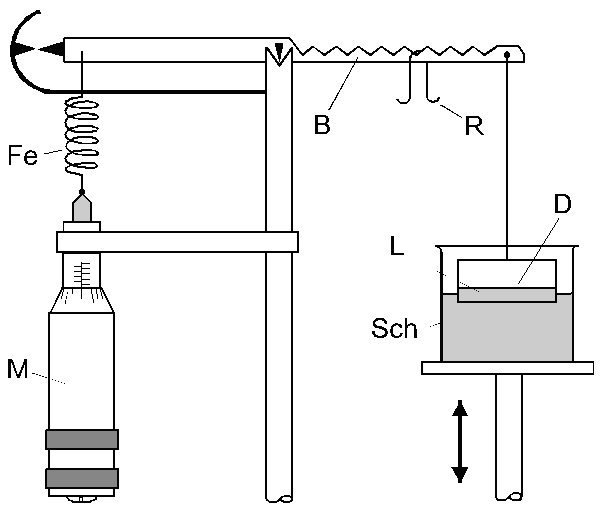
\includegraphics[width=200pt]{fotos/gpr1/screenshot001}
		\caption[Bügelmethode]{Bügelmethode; Fe = Feder; B = Balken; M = Messschraube; L = Flüssigkeitslamelle; Sch = Glasschälchen; D = Messdraht\\ Quelle: \cite{Muller.f}}
		\label{Abb: Versuchsaufbau Bügelmethode}
	\end{figure}
	Weitere Informationen sind im Versuchsskript\smartcite{Muller.f} angegeben.
	
	
	
	\newpage
	\section{Versuchsdurchführung und Auswertung}
		% übersichtliche Darstellung der Messdaten, Rechenergebnisse (chronologische Reihenfolge), Grafiken etc.
		
		\subsection{Kalibrierung}

		
			\begin{figure}[ht!]
			\centering
			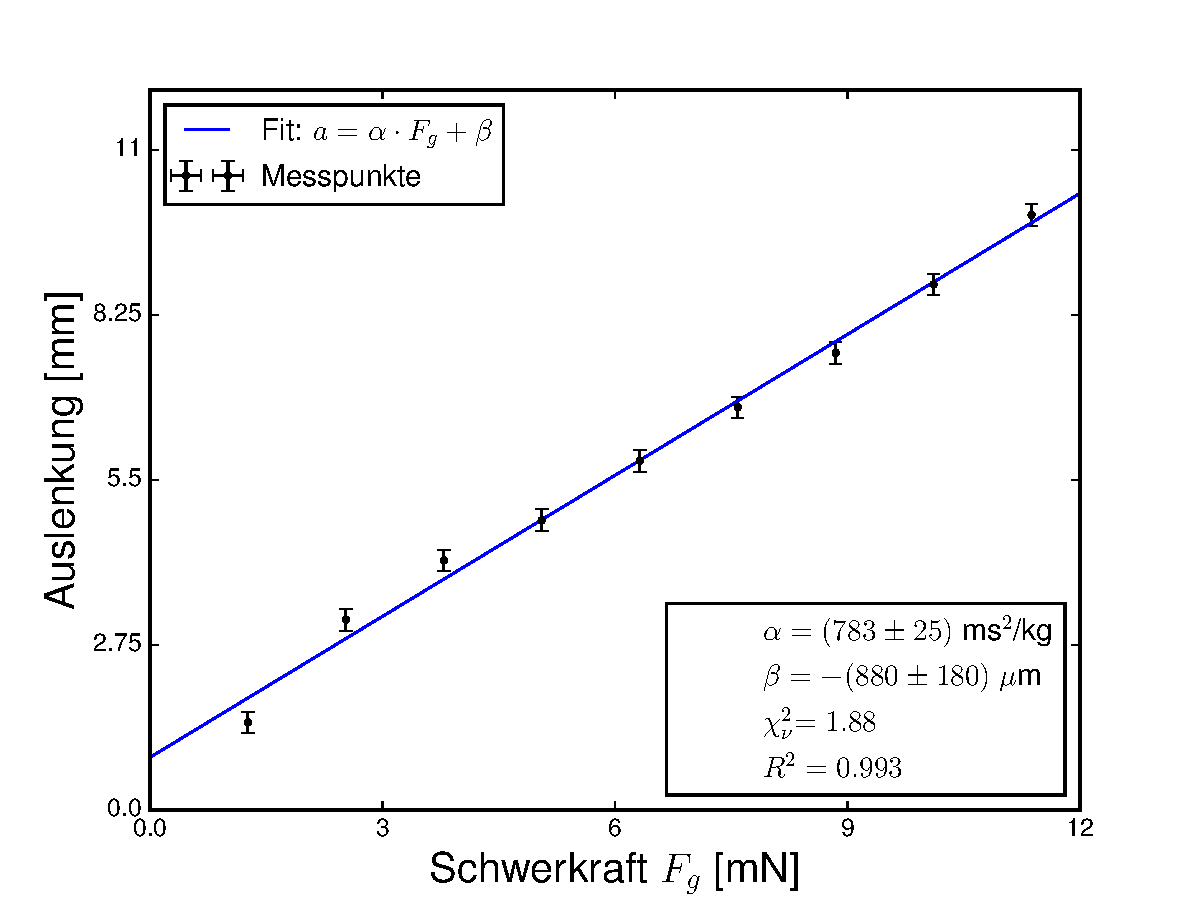
\includegraphics[width=300pt]{fotos/gpr1/M5_Hinweg.pdf}
			\caption[Regression 1]{lineare Regression zwischen Auslenkung $ a $ und der Gewichtskraft $ F_{g} $. Messpunkte sind an den einzelnen Kerben von 1 bis 9 (Hinweg, Zählung von 1, 2,..,9) in Abbildung (\ref{Abb: Versuchsaufbau Bügelmethode}) gemacht worden. }
			\label{Abb: Hinweg}
		\end{figure}
		
		
		\begin{figure}[ht!]
			\centering
			\includegraphics[width=300pt]{fotos/gpr1/M5_Rückweg.pdf}
			\caption[Regression 2]{lineare Regression zwischen Auslenkung $ a $ und der Gewichtskraft $ F_{g} $. Messpunkte sind an den einzelnen Kerben von 1 bis 8 (Rückweg, Zählung 8,7,...,1) in Abbildung (\ref{Abb: Versuchsaufbau Bügelmethode}) gemacht worden. Die Messung an der rechten Kerbe (i=9) wurde ignoriert.}
			\label{Abb: Rückweg}
		\end{figure}
	
	\newpage
	Wir hängen eine kleine Masse ($ R=1.288 $ g) bei der ersten Messung an keine der Kerben und danach vom Drehpunkt nach außen in jede Kerbe $ (i=1,...,9) $ und gleichen den Höhenunterschied zwischen den Spitzen mit der Messschraube aus. Dazu siehe die Abb. (\ref{Abb: Versuchsaufbau Bügelmethode}). \\Die Kalibrierung der Feder machen wir, um die Federkonstante zu brechnen, welche wir in der Bügelmethode brauchen, um die Kraft zu berechnen. Hierzu haben wir folgende Formel verwendet:
	\begin{equation}\label{eq: Federkonstante k}
		k=\dfrac{1}{\alpha}
	\end{equation}
Dabei bezeichnet $ k $ die Federkonstante und $ \alpha $ den jeweiligen Anstieg der linearen Regression in den Abbildungen (\ref{Abb: Hinweg}) und (\ref{Abb: Rückweg}). Die Unsicherheit von $ k $ haben wir mittels Gauß'scher Fehlerfortpflanzung berechnet.
		\begin{equation}\label{eq: Fehler Federkonstante}
			u_{k}=\sqrt{\left(-\dfrac{1}{\alpha^{2}}\cdot u_{\alpha}\right)^{2}}
		\end{equation}
	Somit kommen wir zu folgenden Ergebnissen für die Federkonstanten:

    \begin{table}[H]
			\centering
			\caption[Ergebnisse der Kalibrierung]{Ergebnisse der Kalibrierung; \\indirekt gemessene Federkonstante}
			\begin{tabular}{|c|c|}
				\hline
				Platz 4 & \textbf{Federkonstante} [kg s$ ^{-2} $]\\
				\hline
				\textbf{Hinweg} &  $ 1.28\pm 0.04 $\\
				\hline
				\textbf{Rückweg} & $ 1.235 \pm 0.023 $ \\
				\hline
			\end{tabular}
			\label{tab: Federkonstante}
		\end{table}
		
		
		
	\subsection{Bügelmethode}
Der Versuch wird, wie in Kapitel \ref{sect: Bügelmethode} beschrieben, durch geführt. Um die aus den Messwerten die Oberflächenspannung zu berechnen, verwenden wir folgende Formel:
\begin{equation}\label{eq: Oberflächenspannung 1}
	\sigma=\dfrac{F}{2l}
\end{equation}
Für die Kraft $ F $ gilt $ F=x k $, sodass für $\sigma$ gilt:
\begin{equation}\label{eq: Oberflächenspannung 2}
	\sigma=\dfrac{xk}{2l}
\end{equation}
$ x $ ist die Auslenkung,%$ ^{\ref{Abb: Versuchsaufzeichungen Seite 2}} $, 
die mithilfe der Messchraube gemessen wurde. $ k $ ist die oben berechnete Federkonstante und $ l = (50.5\pm 0.5)$ mm%$ ^{\ref{Abb: Versuchsaufzeichungen Seite 1}} $ 
ist die Länge des Drahtes.\\
Die Unsicherheit der Oberflächenspannung haben wir mittels Gauß'scher Fehlerfortpflanzung wie folgt berechnet:
\begin{equation}\label{eq: Fehler sigma}
	u_{\sigma}=\sqrt{u_{k}^{2}\left(\dfrac{x}{2l}\right)^{2}+u_{x}^{2}\left(\dfrac{k}{2l}\right)^{2}+u_{l}^{2}\left(-\dfrac{x}{2l^{2}}\right)^{2}}
\end{equation}
\newpage
Die Bedeutungen der Variablen in der Gleichung (\ref{eq: Fehler sigma}) lauten wie folgt:

\begin{itemize}
	\item[$ x $] Auslenkungsdifferenz zwischen dem Draht unter dem Wasser und dem Draht über \\dem Wasser
	\item[$ l $] Länge des Drahtes ($ l=50.5 $mm)
	\item[$ k $] Federkonstante
	\item[$ u_{l} $] Unsicherheit der Länge des Drahtes ($ u_{l}=0.5 $mm)
	\item[$ u_{x} $] Unsicherheit der Auslenkungsdifferenz ($ u_{x}=0.13 $mm)
	\item[$ u_{k} $] Unsicherheit der Federkonstante
\end{itemize}
\begin{table}[H]
	\centering
	\caption[Oberflächenspannung]{indirekt gemessenes Ergebnis: Oberflächenspannung}
	\begin{tabular}{|c|c|}
		\hline
		&Platz 4  \\
		\hline
		\textbf{Oberflächenspannung} [mN$ \cdot $m$ ^{-1} $ ]& $ (65\pm 3) $ \\
		\hline
	\end{tabular}
	\label{tab: Ergebnis Oberf.sp.}
\end{table}


Für die Berechnung der Oberflächenspannung haben wir $ x $ gemittelt.


	
	
	
	\subsection{Chi Quadrat}
	
	\begin{table}[H]
    \centering
		\caption{$\chi^{2}$ Ergebnisse}
		\begin{tabular}{|c|c|}
			\hline
			Platz 4 &  $\chi^{2}$\\
			\hline
			\textbf{Hinweg} & 1.88 \\
			\hline
			\textbf{Rückweg} &  0.45\\
			\hline
		\end{tabular}
		\label{tab: Ergebnisse chi quadrat}
\end{table}
	
	Für beide Regressionen passt die lineare Regression als Modell. Dennoch zeigen die $ \chi^{2}_{\nu} $e, dass wir nicht alle physikalischen Vorgänge im Experiment berücksichtigt haben. Aus dem zweiten reduzierten $ \chi^{2} $ können wir schließen, dass wir die Fehler minimal zu groß gewählt haben. Dies könnte jedoch auch Rudungsfehler sein. Eine klare Aussage ist aufgrund der Größe der $ \chi^{2} $e ist nicht möglich, ob es sich um statistische Schwankungen oder um andere Einflüsse handelt.\smartcite{Grimm.13.07.2021} Beim ersten reduzierten $ \chi^{2} $ können wir die Vermutung im Kapitel (\ref{sect: Fehlerabschätzung Kalibrierung}) erhärten, dass die Oberflächenspannung einen Einfluss auf die Kalibrierung der Feder hatte. Schlussendliche können wir die reduzierten $ \chi^{2} $ nicht ablehnen. Eine Veranschaulichung der $ \chi^{2} $e in Bezug auf die Konfidenzintervalle liefert die Abbildung (\ref{Abb: Chi Quadrate})
	
	
	\newpage
	\section{Fehlereinschätzung}
% gründliche Analyse der aufgetretenen Messabweichungen und ihre Ursachen

\subsection{Oberflächenspannung bei Kalibrerung}\label{sect: Fehlerabschätzung Kalibrierung}
Der Draht, welchen man in der Abb. (\ref{Abb: Versuchsaufbau Bügelmethode}) bei D sehen kann, befand sich am Anfang der Kalibrierung knapp unter der Wasseroberfläche. Während der Messung ist der Draht dann über die Wasseroberfläche gelangt und die Oberflächenspannung hat den Draht entsprechend zurückgehalten bis sich die Lamelle vom Draht gelöst hat. Aufgrund dessen ist am Anfang der ersten Messreihe (Abb. (\ref{Abb: Hinweg})) ein Sprung zu sehen, welcher sich eben auf die Oberflächenspannung zurückführen lässt. Jedoch ist der Fehler nicht berücksichtigt worden.
\subsection{Ablesefehler}
\begin{table}[H]
    \centering
	\caption{Unsicherheiten bzgl. Messschraube \& Spitzen}
	\begin{tabular}{|c|c|}
		\hline
		& Unsicherheit \\
		\hline
		Ablesefehler, Messschraube & 0.005 mm \\
		\hline
		Ablesefehler, Spitzen & 0.130 mm \\
		\hline
	\end{tabular}
	\label{tab: u_M und u_S}
\end{table}


Der Ablesefehler von der Messschraube wurde in den Rechnungen nicht berücksichtigt, weil sie im Vergleich zu einem kleinen aber deutlichen Höhenunterschied zwischen den Spitzen in Abb. (\ref{Abb: Versuchsaufbau Bügelmethode}) geringer ist. Stattdessen wurde die Differenz einer deutlichen Veränderung der beiden Spitzen über der Feder (Fe) (siehe Abb. (\ref{Abb: Versuchsaufbau Bügelmethode})) gemessen und als Fehler verwendet. Den Unterschied sieht der Leser in der Tabelle (\ref{tab: u_M und u_S}). Die Unsicherheit der Messschraube ist eine Abschätzung der Skaleneinteilung. Ich bin davon ausgegangen, dass der Ablesefehler bei etwa einer halben Skaleneinteilung liegt.


	
	\section{Schlussfolgerung}
	% Diskussion über Versuchsergebnisse und Versuchsaufbau
	% ergebnisse mit Referenzwerten unter angaben von Quellen vergleichen
	% experimentele Methoden und Messverfahren  kritisch beobachten und diskutieren, Schlussfolgerungen gezogen werden
	
	Der Versuch ist um einiges umfangreicher als hier dargestellt. Während des Experimentierens hatten, wir nur eine Stunde Zeit, deshalb konnten wir den Versuch nicht vollständig durchführen. Die Bügelmethode konnte nur geringfügig durchgeführt werden und die Kapillarsteighöhenmethode konnte nicht durchgeführt werden.
	\begin{table}[H]
    \centering
		\caption[Vergleich]{Vergleich des gemittelten Messwertes mit \\Referenzdaten aus dem Internet und Literatur, Temperatur: $ 20^{\circ} $C}
		\begin{tabular}{|c|c|}
			\hline
			& Oberflächenspannung [mN$ \cdot $m$ ^{-1} $ ] \\
			\hline
			Messwert & $65\pm 3  $ \\
			\hline
			\hline
			Internet &  72.75\\
			\hline
			Literatur & 72.8 \\
			\hline
		\end{tabular}
		\label{tab: Vergleich}
\end{table}
	
	

	Um das Ergebnis der Oberflächenspannung (\ref{tab: Ergebnis Oberf.sp.}) einschätzen zu können, haben wir aus dem Internet\smartcite{Unbekannt.09.07.2021} und aus der Literatur\smartcite[vgl.][88]{Eichler.2016} Vergleichswerte herangezogen. Eine Ungenauigkeit der Vergleichswerte konnte hingegen nicht gefunden werden, sodass eine vollständige Einschätzung des Ergebnisses nicht möglich ist. Jedoch können wir sagen, dass mit einbeziehen des Fehlers unser Ergebnis sehr nahe an die Vergleichswerte herankommt.  \\\\
	Es wurde vom Versuchsleiter mehrmals darauf aufmerksam gemacht, dass der Draht D (Abb. (\ref{Abb: Versuchsaufbau Bügelmethode})) nicht ins Wasser gelangen sollte. Jedoch wurde schlussendlich nicht darauf geachtet. Dies hat zur Folge, dass die Oberflächenspannung die Messung der Federdkonstanten stark beeinflusst.\footnote{Diese Fehlerbetrachtung bezieht sich nur auf die erste lineare Regression (Abb. (\ref{Abb: Hinweg}))} Eine Abschätzung des Fehlers durch die Oberflächenspannung konnte ich nicht durchführen. Die Ergebnisse lassen vermuten, dass die Oberflächenspannung am Anfang der Kalibrierung keine unherhebliche Rolle gespielt haben muss. Die Temperatur hatte in diesem Versuch auch ihren Einfluss gehabt. Jedoch wurde die Temperatur auf  $ (22^{\circ}\pm 2^{\circ}) $C abgeschätzt. Durch die Schätzung und durch die fehlende Messung der Temperatur ist auch keine Fehlerabschätzung der Temperatur möglich. Desweiteren wäre es von nutzen gewesen, aus zu probieren, ob ein Eintauchen in das destillierte Wasser überhaupt bessere Werte liefert. Ein Vergleich ohne einhängen des Bügels in das destillierte Wasser hätte zeigen können, welche Methode besser geeignet wäre. \\
	\\
	
	Bei der Bügelmethode wäre es gut gewesen, mehr Messreihen aufzunehmen, um ein genaueres Ergebnis zu erlangen. Zudem haben wir mechanische Einflüsse, wie Wind oder Erschütterungen, nicht beachtet, weil die nötigen Messgeräte nicht vorhanden waren. Die mechanischen Einflüsse sorgen dafür, dass es zu einem verfrühten Abreißen der Wasseroberfläche von der Limelle kommt. Daraus folgt, dass die Ergebnisse unter dem eigentlichen wahren Wert liegen. Somit ist das Ergebnis so zu interpretieren, dass die Oberflächenspannung von $ \sigma=(65\pm 3) $mN$ \cdot $m$ ^{-1} $ eine untere Schranke darstellt.
	
	
	
	\newpage
    \appendix
	\section{Anhang}
	
	
	\subsection{Beantwortung der Fragen}
	Die Fragen sind auf der letzten Seite des Versuchsskript zu finden.\smartcite{Muller.f} Wir beanworten im folgenden nur die ersten drei Fragen.
	\subsubsection[Frage 1]{In welcher Weise ist die Oberflächenspannung von der Temperatur abhängig?}\label{sect: Frage 1}
	Wir können die Arbeitsdifferenz in (\ref{eq: Oberflächenspannung}) als die Arbeit aus dem ersten Hauptsatz der Thermodynamik betrachten:\smartcite[vgl.][148]{Eichler.2016}
	\begin{equation}\label{eq: Arbeit=innere Energie-Wärme}
		\Delta W= \Delta U-Q
	\end{equation}
Die innere Energie $  U$ wiederum können wir als multiplikativen Zusammenhang zwischen der mittleren kinetische Energie $ \overline{E}_{kin} $ und der Anzahl $ N $ von Teilchen betrachten:
\begin{equation}\label{eq: innere Energie}
	U=\overline{E}_{kin} N
\end{equation}
	und die mittlere kinetische Energie $ \overline{E}_{kin} $ ist von der Temperatur $ T $ abhängig:\smartcite[vgl.][117]{Eichler.2016}
	\begin{equation}\label{eq: Ekin}
		\overline{E}_{kin}=\dfrac{3}{2}k T
	\end{equation}
Als $ k $ wird hier die Boltzmann Konstante bezeichnet.\smartcite[vgl.][117]{Eichler.2016}
	\subsubsection[Frage 2]{Warum nehmen Flüssigkeitstropfen oder Gasbläschen Kugeltropfen an?}\label{sect: Frage 2}
	Die Kugelform hat die gerinste Oberfläche.\smartcite{Unbekannt.04.07.2021} Dies ist damit zu begründen, dass sich die Oberfläche auf ein Minimum zusammenzieht, um auf die geringste potentielle Energie zu kommen.\smartcite{Muller.f}
	
	
	
	\subsubsection[Frage 3]{Welche alternativen Methoden (außerhalb des Versuchsskripts) sind zur Messung von Oberflächenspannungen geeignet?} \label{sect: Frage 3}
	\textit{Du-Noüy-Ringmethode:}\\
	<<Gemessen wird die Kraft  einer vom Ring hochgezogenen Flüssigkeitslamelle.>>\smartcite{Unbekannt.04.07.2021}\\
	\\
	\textit{Wilhelmy-Plattenmethode:}\\
	<<Gemessen wird die Kraft, die sich durch die Benetzung der senkrecht aufgehängten Platte ergibt.>>\smartcite{Unbekannt.04.07.2021}\\
	\\
	\textit{Pendant-Drop-Methode:}\\
	<<Optische Erfassung der Tropfengeometrie. Größe der Tropfen, die von einer Kapillare abtropfen, ist proportional zur Oberflächenspannung.>>\smartcite{Unbekannt.04.07.2021}
	
	
	
	\newpage
	\subsection{Weiterführende Abbildungen}
		\begin{figure}[ht!]
		\centering
		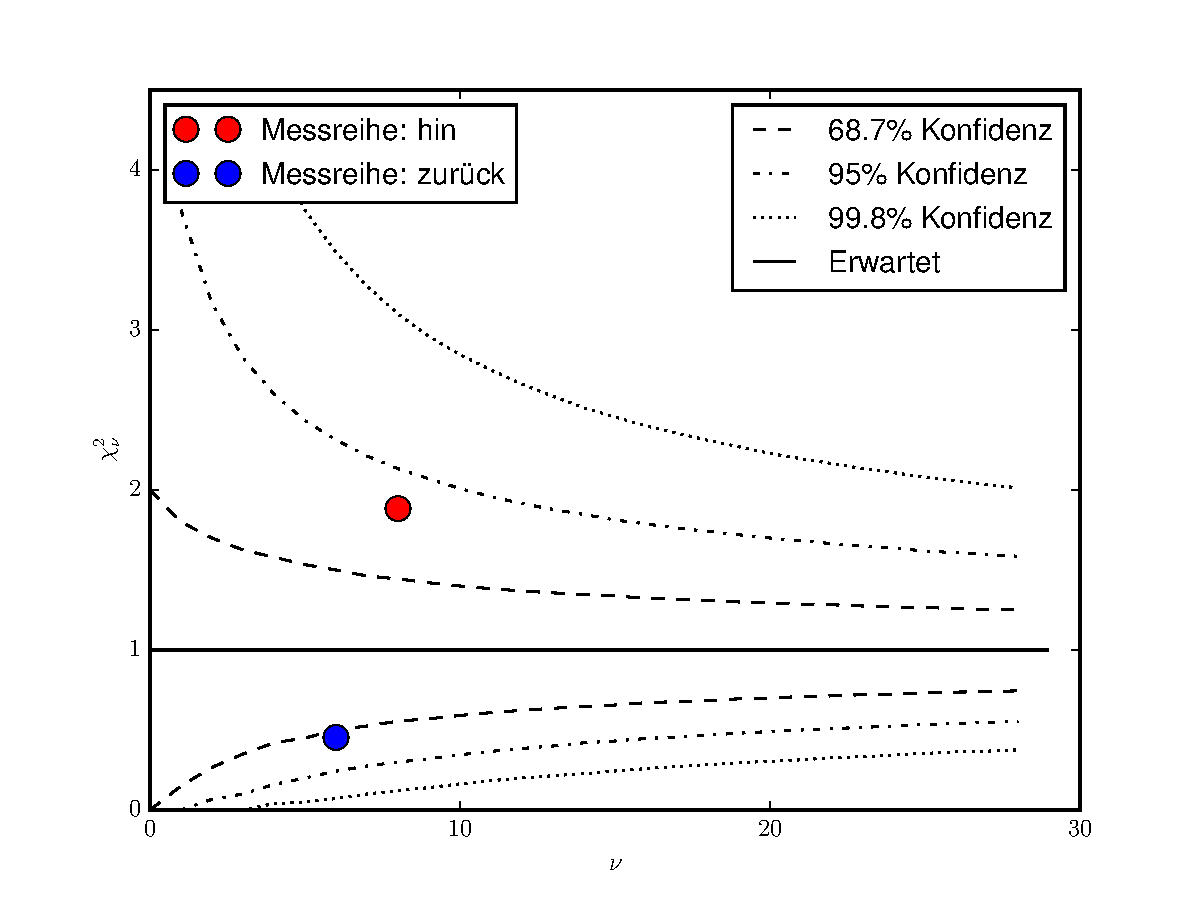
\includegraphics[width=450pt]{fotos/gpr1/M5_Chi_Quadrat.pdf}
		\caption[reduzierte Chi Quadrate]{reduzierte $  \chi^{2} $e von der Kalibrierung der Feder. \\Reduziertes $  \chi^{2} $ in Abhängigkeit der Freiheitsgrade $ \nu $}
		\label{Abb: Chi Quadrate}
	\end{figure}

Im folgenden habe ich für die Nachbesprechung die Abbildung (\ref{Abb: Hinweg}) nochmal überarbeitet. Aus den linearen Regressionen habe ich die Federkonstanten bestimmt und mit deren Hilfe die Oberflächenspannungen bestimmt. Beide Werte habe ich jeweils in eine Tabelle unter die jeweilige Grafik angegeben. Das Endergebnis habe ich jedoch nicht weiter verbessert.

\newpage

\begin{figure}[ht!]
	\centering
	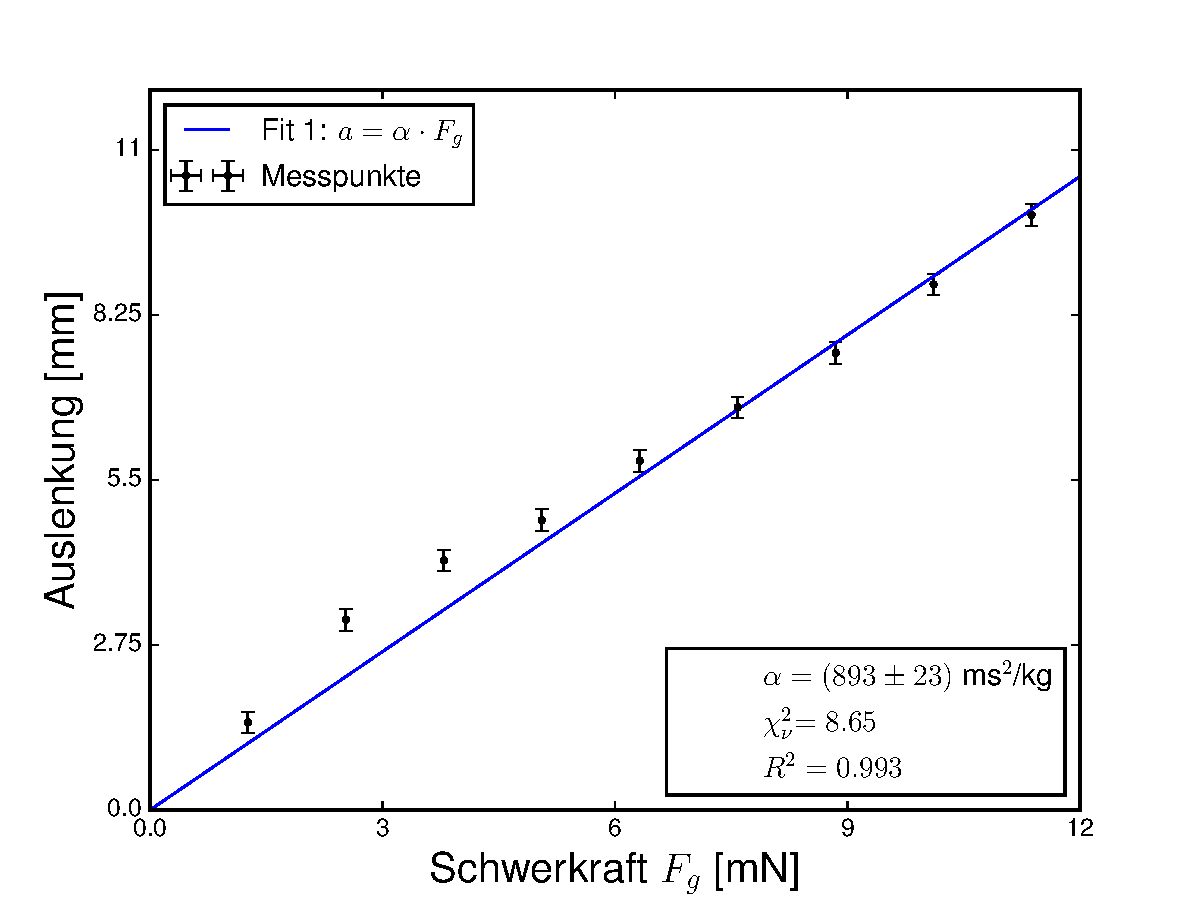
\includegraphics[width=400pt]{fotos/gpr1/M5_Hinweg_1.pdf}
	\caption[Regression 1 Korrektur 1]{lineare Regression zwischen Auslenkung $ a $ und der Gewichtskraft $ F_{g} $. Messpunkte sind an den einzelnen Kerben von 1 bis 9 (Hinweg, Zählung von 1, 2,..,9) in Abbildung gemacht worden. }
	\label{Abb: Hinweg1}
\end{figure}
\begin{table}[ht!]
	\centering
	\caption{Ergebnisse}
	\begin{tabular}{|c|c|}
		\hline
		& Platz 4 \\
		\hline
		Federkonstante [kg s$ ^{-2} $]& $k_{2}= 1.120\pm0.028 $ \\
		\hline
		Oberflächenspannung [mN$ \cdot $m$ ^{-1} $ ]& $\sigma_{2}= 58\pm 5$ \\
		\hline
	\end{tabular}
	\label{tab: Erg 2}
\end{table}


\newpage
\begin{figure}[ht!]
	\centering
	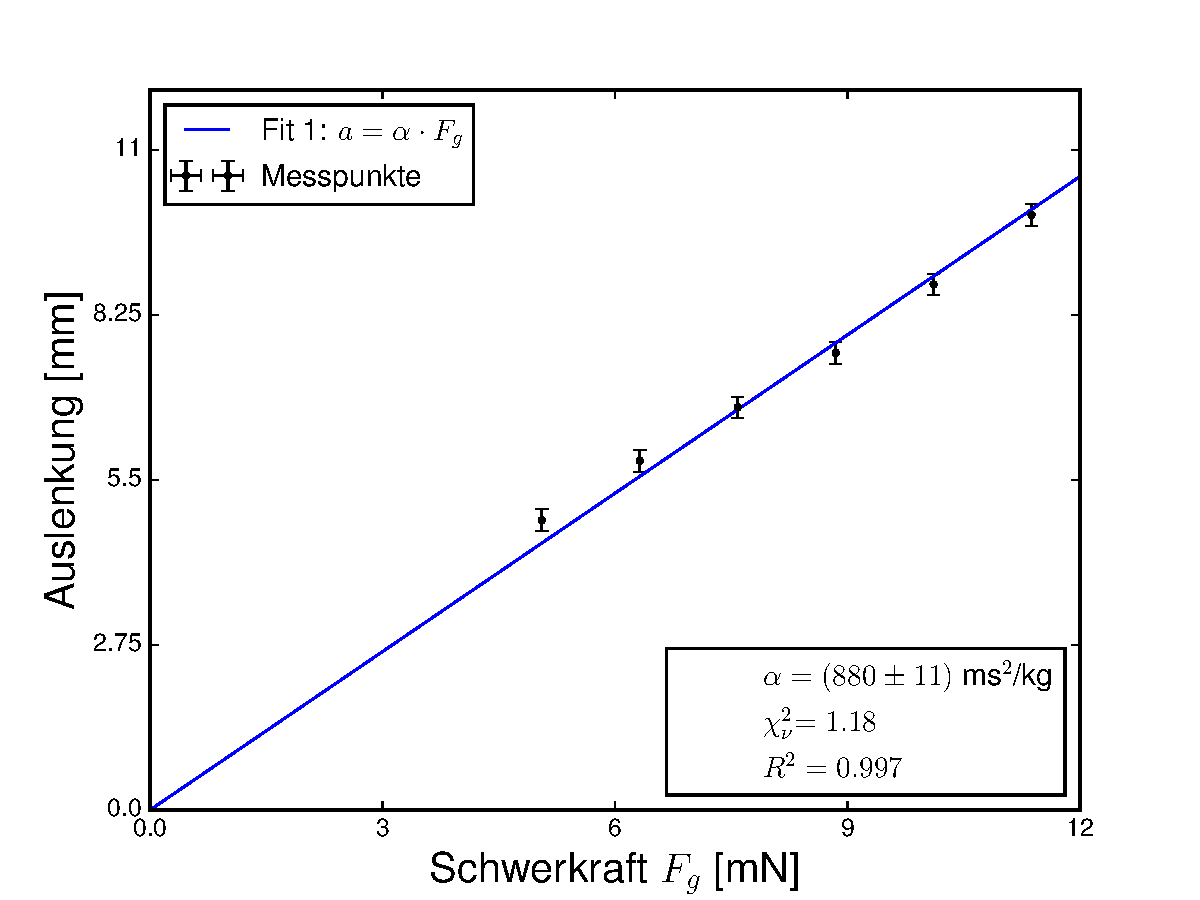
\includegraphics[width=400pt]{fotos/gpr1/M5_Hinweg_2.pdf}
	\caption[Regression 1 Korrektur 2]{lineare Regression zwischen Auslenkung $ a $ und der Gewichtskraft $ F_{g} $. Messpunkte sind an den einzelnen Kerben von 1 bis 9 (Hinweg, Zählung von 1, 2,..,9) in Abbildung gemacht worden. }
	\label{Abb: Hinweg2}
\end{figure}
\begin{table}[ht!]
	\centering
	\caption{Ergebnisse}
	\begin{tabular}{|c|c|}
		\hline
		& Platz 4 \\
		\hline
		Federkonstante [kg s$ ^{-2} $]& $k_{3}=1.136\pm 0.014  $ \\
		\hline
		Oberflächenspannung [mN$ \cdot $m$ ^{-1} $ ]& $\sigma_{3}= 59\pm 5 $ \\
		\hline
	\end{tabular}
	\label{tab: Erg 3}
\end{table}

\newpage
	\printbibliography[title={Quellenverzeichnis}]
	
	
\end{document}